\documentclass[
  journal=small,
  manuscript=Reporte-de-laboratorio-computacional,  % Use a - if you need a space e.g. "research-article"
  year=2023,
  volume=Febrero,
]{cup-journal}

\usepackage{amsmath} 
\usepackage[nopatch]{microtype}
\usepackage{booktabs}

\title{Aplicación de la regla del trapecio para integrales dobles en un problema físico.}

\author{Jesús Eduardo Loera Casas}
\affiliation{Facultad de Ciencias Físico Matemáticas, San Nicolás de 
los Garzas, Nuevo León, México}
\email[J. Loera]{colab.git@gmail.com}

%\author{S. Author}
%\affiliation{Second Division, Organization, City, Pincode, State, Country}
% \alsoaffiliation{Joint first authors}

%\author{T. Author}
%\affiliation{Second Division, Organization, City, Pincode, State, Country}

%\author{F.T. Author}
%\affiliation{Fourth Division, Organization, City, Pincode, State, Country}

\addbibresource{example.bib}

\keywords{Integración numérica, Método de Romberg, Método de Extrapolación de Richardson, Fortran, Python} 

\begin{document}

\begin{abstract}
    En este reporte implementamos el método de Romberg y el método de extrapolación de Richardson en los lenguajes de Fortran y Python. El método funciona para resolver integrales definidas de funciones de una variable real. Una vez implementado el método, este se aplicó para resolver la ecuación del cohete, donde se mostró que el método de extrapolación de Richardson es eficiente para iterar los resultados numéricos de obtenidos con el método de Romberg y mejorar la precisión de las integrales calculadas.
\end{abstract}

\section{Introducción}

\noindent En prácticamente todas las ramas de la física la integración tiene un papel muy importante, conocemos muchas magnitudes físicas cuya definición implica una integral, particularmente el flujo eléctrico, el flujo magnético y la normalización de la función de onda bidimensional son ejemplos de definiciones que implican una integral doble.

\begin{equation*}
  \braket{\psi | \psi} = \displaystyle\int_{S} \psi^{*} \psi dA
\end{equation*}

\begin{equation*}
  \Phi_B = \displaystyle\int_{S} \vec{B} \cdot  d\vec{A}
  \quad \quad \quad
  \Phi_E = \displaystyle\int_{S} \vec{E} \cdot  d\vec{A}
\end{equation*}

El cálculo de dichas integrales se puede volver complicado, por ello solemos recurrir a técnicas de integración numérica para resolver el problema de manera computacional.

\section{El Método de Romberg}

\vspace{0.5cm}

El método de Romberg (\cite{scherer2010computational}) es un método de integración numérica que permite calcular el valor aproximado de las integrales de la forma

\begin{equation*}
    I = \displaystyle\int_{a}^{b} f(x)dx
\end{equation*}

\noindent donde f(x) es una función escalar de una variable real X.

\vspace{0.5cm}

\noindent \textbf{El algoritmo de Romberg}

\vspace{0.5cm}

El método de Romberg consiste en discretizar el intervalo $\left[a,b\right]$ en una malla de puntos equidistantes de manera que la distancia que separa a dos puntos contiguos está dada por 

\begin{equation*}
    h_n = \frac{b-a}{2^{n-1}}
\end{equation*}

\noindent en donde $n \ge 1 $ y $ m \ge 1$.

\vspace{0.5cm}

Este es un método iterativo y recursivo, donde $R_{n,m}$ representa la aproximación a la integral numérica con un error del orden $O(h_{n}^{2m+1})$. Podemos encontrar el valor de $R_{n,m}$ de la siguiente manera:

\begin{equation*}
    R_{1,1} = \frac{1}{2} \left(b-a\right) (f\left(a\right) + f\left(b\right))
\end{equation*}

\begin{equation*}
    R_{n,1} = \frac{h_n}{2} \left[ f\left( a \right) + f\left(b\right) + 2 \displaystyle\sum_{i=1}^{2^{n-1}} f\left(a+ih_n\right) \right]
\end{equation*}

\begin{equation*}
    R_{i,j} = \frac{ 4^{ j-1 } R_{ i, j-1} - R_{ i-1, j-1} }{ 4^{ j-1} -1}
\end{equation*}

El corazón del método de Romberg es el \emph{método de Extrapolación de Richardson}, un método que toma una secuencia convergente para construir otra secuencia que converge más rápido. Este es ampliamente utilizado en un sin fin de métodos numéricos interativos, pero su más icónica aplicación es justamente en la construcción del algoritmo de Romberg.


%\subsection{El Método de Extrapolación de Richardson}
Subsection text here. Lorem ipsum\autocite{Bayer_etal_2013} dolor sit amet, consectetur adipiscing elit, sed do eiusmod tempor incididunt ut labore\autocite{Adade_etal_2007} et dolore magna aliqua. 

 Lorem ipsum dolor sit amet, consectetur adipiscing elit, sed do eiusmod tempor incididunt ut labore et dolore magna aliqua. Lorem ipsum dolor sit amet, consectetur adipiscing elit, sed do eiusmod tempor incididunt ut labore et dolore magna aliqua. Lorem ipsum dolor sit amet, consectetur adipiscing elit, sed do eiusmod tempor incididunt ut labore et dolore magna aliqua. 


\subsubsection{Resolver la ecuación del Cohete}

\vspace{0.5cm}

\noindent \textbf{Problema.} The upward velocity of a rocket can be computed by the following formula:

\begin{equation*}
    v = u ln\left(\frac{m_o}{m_o -qt}\right) -gt
\end{equation*}

\noindent where $v = \textnormal{upward velocity} $,  $u = \textnormal{velocity at which fuel is expelled relative to the rocket}$, $m_o = \textnormal{initial mass of the rocket at time} $ $t=0$,  $q = \textnormal{fuel consumption rate}$, and $g = \textnormal{downward acceleration of gravity}$ (assumed constant = $9.8 m/s^2 $). If $u=1800m/s$, $m_o=160000kg$ and $q=2500kg/s$, use six-segment trapezoidal and Simpson's $1/3$ rule, six-point Gauss quadrature, and $O(h^8)$ Romberg mehtods to determine how high the rocket will fly in 30 s.

\begin{itemize}
    \item Solución con Python
\end{itemize}

\begin{figure}[h!]
    \centering
    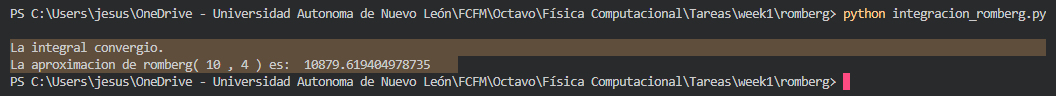
\includegraphics[width=1\linewidth]{images/python.png}
    \caption{Se ejecutó el script de Python que resuelve el problema físico.}
    \label{fig_python}
\end{figure}

\begin{itemize}
    \item Solución con Fortran
\end{itemize}

\begin{figure}[H]
    \centering
    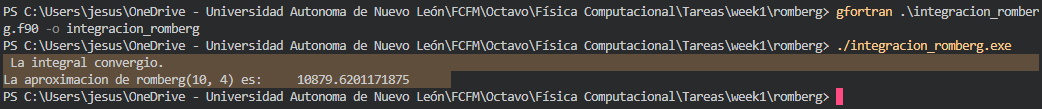
\includegraphics[width=1\linewidth]{images/fortran.png}
    \caption{Se ejecutó el script de Python que resuelve el problema físico.}
    \label{fig_fortran}
\end{figure}

Vea una comparación de las respuestas obtenidas en cada script en la tabla~\ref{table_results}.

\begin{table}[hbt!]
    \begin{threeparttable}
    \caption{Se resolvió el problema de la altura alcanzada por el cohete con el script en Python y Fortran.}
    \label{table_results}
    \begin{tabular}{ll}
    \toprule
    \headrow  & Altura alcanzada en 30 segundos \\
    \midrule
    Python & 10879.61940497 metros \\ 
    \midrule
    Fortran & 10879.62011718 metros \\ 
    \bottomrule
    \end{tabular}
\end{threeparttable}
\end{table}

%\section{Equations}

Sample equations. Lorem ipsum dolor sit amet, consectetur adipiscing elit, sed do eiusmod tempor incididunt ut labore et dolore magna aliqua. Lorem ipsum dolor sit amet, consectetur\endnote{Another footnote/endnote} adipiscing elit, sed do eiusmod tempor incididunt ut labore et dolore magna aliqua. Lorem ipsum dolor sit amet, consectetur adipiscing elit, sed do eiusmod tempor incididunt ut labore et dolore magna aliqua. 


%%% Numbered equation
\begin{equation}
\begin{aligned}\label{eq:first}
\frac{\partial u(t,x)}{\partial t} = Au(t,x) \left(1-\frac{u(t,x)}{K}\right)
 -B\frac{u(t-\tau,x) w(t,x)}{1+Eu(t-\tau,x)},\\
\frac{\partial w(t,x)}{\partial t} =\delta \frac{\partial^2w(t,x)}{\partial x^2}-Cw(t,x)
+D\frac{u(t-\tau,x)w(t,x)}{1+Eu(t-\tau,x)},
\end{aligned}
\end{equation}

 Lorem ipsum dolor sit amet, consectetur adipiscing elit, sed do eiusmod tempor incididunt ut labore et dolore magna aliqua. Lorem ipsum dolor sit amet, consectetur adipiscing elit, sed do eiusmod tempor incididunt ut labore et dolore magna aliqua. Lorem ipsum dolor sit amet, consectetur adipiscing elit, sed do eiusmod tempor incididunt ut labore et dolore magna aliqua. 

\begin{align}\label{eq:another}
\begin{split}
\frac{dU}{dt} &=\alpha U(t)(\gamma -U(t))-\frac{U(t-\tau)W(t)}{1+U(t-\tau)},\\
\frac{dW}{dt} &=-W(t)+\beta\frac{U(t-\tau)W(t)}{1+U(t-\tau)}.
\end{split}
\end{align}


%%%% Unnumbered equation
\begin{align*}
&\frac{\partial(F_1,F_2)}{\partial(c,\omega)}_{(c_0,\omega_0)} = \left|
\begin{array}{ll}
\frac{\partial F_1}{\partial c} &\frac{\partial F_1}{\partial \omega} \\\noalign{\vskip3pt}
\frac{\partial F_2}{\partial c}&\frac{\partial F_2}{\partial \omega}
\end{array}\right|_{(c_0,\omega_0)}\\
&\quad=-4c_0q\omega_0 -4c_0\omega_0p^2 =-4c_0\omega_0(q+p^2)>0.
\end{align*}

%
\section{Figures \& Tables}

The output for a single-column figure is in Figure~\ref{fig_sim}.  Lorem ipsum dolor sit amet, consectetur adipiscing elit, sed do eiusmod tempor incididunt ut labore et dolore magna aliqua. Lorem ipsum dolor sit amet, consectetur adipiscing elit, sed do eiusmod tempor incididunt ut labore et dolore magna aliqua. Lorem ipsum dolor sit amet, consectetur adipiscing elit, sed do eiusmod tempor incididunt ut labore et dolore magna aliqua. 

Lorem ipsum dolor sit amet, consectetur adipiscing elit, sed do eiusmod tempor incididunt ut labore et dolore magna aliqua. Lorem ipsum dolor sit amet, consectetur adipiscing elit, sed do eiusmod tempor incididunt ut labore et dolore magna aliqua. Lorem ipsum dolor sit amet, consectetur adipiscing elit, sed do eiusmod tempor incididunt ut labore et dolore magna aliqua. 

%See Figure~\ref{fig_wide} for a double-column figure; this is always at the top of a following page.


\begin{figure}[hbt!]
\centering
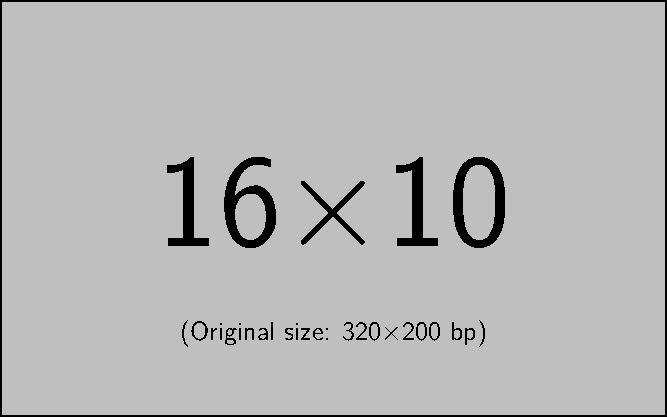
\includegraphics[width=0.75\linewidth]{images/example-image-16x10.pdf}
\caption{Insert figure caption here}
\label{fig_sim}
\end{figure}


\begin{figure*}
\centering
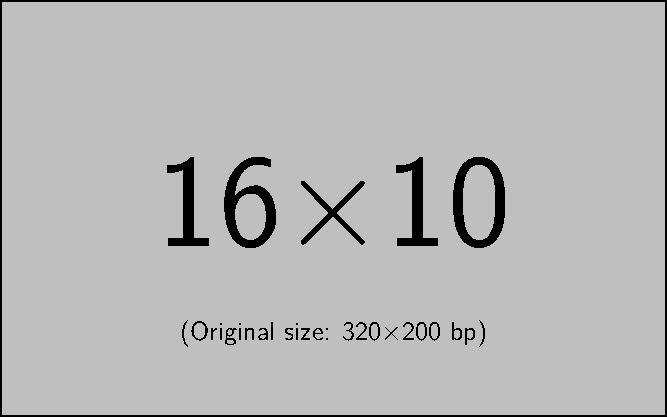
\includegraphics[width=0.8\linewidth]{images/example-image-16x10.pdf}
\caption{Insert figure caption here}
\label{fig_wide}
\end{figure*}


See example table in Table~\ref{table_example}.

\begin{table}[hbt!]
\begin{threeparttable}
\caption{An Example of a Table}
\label{table_example}
\begin{tabular}{llll}
\toprule
\headrow Column head 1 & Column head 2  & Column head 3 & Column head 4\\
\midrule
One\tnote{a} & Two&three three &four\\ 
\midrule
Three & Four&three three\tnote{b} &four\\
\bottomrule
\end{tabular}
\begin{tablenotes}[hang]
\item[]Table note
\item[a]First note
\item[b]Another table note
\end{tablenotes}
\end{threeparttable}
\end{table}


\section{Conclusion}
The conclusion text goes here.


%\begin{acknowledgement}
    Insert the Acknowledgment text here.
    \end{acknowledgement}
    
    \paragraph{Funding Statement}
    
    This research was supported by grants from the <funder-name> <doi> (<award ID>); <funder-name> <doi> (<award ID>).
    
    \paragraph{Competing Interests}
    
    A statement about any financial, professional, contractual or personal relationships or situations that could be perceived to impact the presentation of the work --- or `None' if none exist.
    


%\endnote in some journals will behave like \footnote; and \printendnotes will not output anything. 
%\printendnotes

\printbibliography

\appendix
\section{Programa en Python}

Lorem ipsum dolor sit amet, consectetur adipiscing elit, sed do eiusmod tempor incididunt ut labore et dolore magna aliqua. Lorem ipsum dolor sit amet, consectetur adipiscing elit, sed do eiusmod tempor incididunt ut labore et dolore magna aliqua. Lorem ipsum dolor sit amet, consectetur adipiscing elit, sed do eiusmod tempor incididunt ut labore et dolore magna aliqua. 

\end{document}
\section{Programa en Fortran}

\lstset{language=[90]Fortran,
  basicstyle=\ttfamily\scriptsize,
  keywordstyle=\color{red},
  commentstyle=\color{blue},
  breaklines=true,
  showstringspaces=false,
  morecomment=[l]{!\ }% Comment only with space after !
}

\begin{lstlisting}
        ! Programa elaborado por Jesus Eduardo Loera Casas
        ! Fecha 09/02/23
        
        ! En este programa resolvemos integrales dobles con la regla
        ! del trapecio.
        
                ! definimos el integrandpo 
                real function f(x,y)
                    implicit none
                    real :: x,y
                    f = log(x+2*y)
                    return
                end function
        
                ! programa principal
                program main
        
                    implicit none
                    real :: integral, dx, dy, xo, xf, yo, yf
        
                    ! definimos la region de integracion
                    xo = 1.4 ; xf = 2.0
                    yo = 1.0 ; yf = 1.5
        
                    ! definimos el tamano de subintervalo de integracion
                    dx = 0.0001 ; dy = 0.0001
        
                    call integracion_doble(xo, xf, yo, yf, dx, dy, integral)
        
                    write(*,*) "El valor de la integral es: ", integral
        
                end program main
        
                ! subrutina que calcula la integral doble con regla del trapecio
                subroutine integracion_doble(xo, xf, yo, yf, dx, dy, integral)
                    implicit none
                    real :: xo, xf, yo, yf, dx, dy, integral, suma
                    real :: f
                    real :: trapecio_y, aux
                    integer :: Nx, Ny, i
                    Nx = (xf-xo)/dx + 1
                    Ny = (yf-yo)/dy + 1
                    suma = 0.0
                    do i = 1, Nx-1
                        suma = suma + trapecio_y(yo, yf, dy, xo + i*dx)
                    end do
                    aux = trapecio_y(yo,yf,dy,xo) + trapecio_y(yo,yf,dy,xf)
                    integral = (0.5*dx)*(aux + 2*suma)
                end subroutine
        
                ! regla del trapecio para integrar funciones f(cte,y)
                real function trapecio_y(yo, yf, dy, xcte)
                    implicit none
                    real :: yo, yf, dy, suma
                    ! funcion del integrando
                    real :: f, xcte
                    integer :: N, i
        
                    N = (yf-yo)/dy + 1
                    suma = 0.0
                    do i = 1, N-1
                        suma = suma + f(xcte, yo+i*dy)
                    end do
                    trapecio_y = (0.5*dy)*(f(xcte,yo) + f(xcte,yf) + 2*suma)
        
                    return
                end function
\end{lstlisting}

\end{document}